\documentclass[a4paper]{article}
\usepackage[a4paper,left=2.5cm,right=2cm,top=2.5cm,bottom=2.5cm]{geometry}
\usepackage[utf8]{inputenc}
\usepackage[T1]{fontenc}
\usepackage{textcomp}
\usepackage[english]{babel}
\usepackage{amsmath, amssymb}
\usepackage{natbib}
\usepackage{parskip}
\usepackage{float} 
\usepackage[caption = false]{subfig}
\usepackage{listings}
\lstset{
    breaklines=true,
    basicstyle=\tt\normalsize,
    keywordstyle=\color{blue},
    identifierstyle=\color{magenta},
    frame = single
} 
\usepackage{tcolorbox}
\newtcolorbox{example}[1]{colback=blue!5!white,colframe=blue!75!black,fonttitle=\bfseries,title=#1}
\newtcolorbox{definition}[1]{colback=red!5!white,colframe=red!75!black,fonttitle=\bfseries,title=#1}
\newtcolorbox{wbox}[1]{colback=white!5!white,colframe=black!75!white,fonttitle=\bfseries,title=#1}


%\usepackage{xcolor}
%\usepackage[explicit]{titlesec}


%\definecolor{redbg}{RGB}{235, 214, 214}
%\definecolor{Red}{RGB}{163, 25, 25}
%\definecolor{Black}{RGB}{0, 0, 0}

%\titleformat{\section}
%  {\no
%  {}
%  {0em}
%  {\colorbox{redbg}{\parbox{\dimexpr\textwidth-2\fboxsep\relax}{\textcolor{Red}{\thesection\quad#1}}}}

%Underlining ruler for subsections
%\titleformat{\subsection}
%  {\normalfont\large\bfseries\color{Red}}
%  {\thesubsection}
%  {1em}
%  {#1}
%  [{\titlerule[0.8pt]}]
%  \titlespacing{\subsection}{0pt}{3pt}{3pt}
%  \let\oldtitleline\titleline
%\renewcommand{\titleline}{\oldtitleline*}


% figure support
\usepackage{import}
\usepackage{xifthen}
\pdfminorversion=7
\usepackage{pdfpages}
\usepackage{transparent}
\pdfsuppresswarningpagegroup=1
\usepackage{xifthen}

\def\testdateparts#1{\dateparts#1\relax}
\def\dateparts#1 #2 #3 #4 #5\relax{
    \marginpar{\small\textsf{\mbox{#1 #2 #3 #5}}}
}

\def\@lesson{}%
\newcommand{\lesson}[3]{
    \ifthenelse{\isempty{#3}}{%
        \def\@lesson{Lecture #1}%
    }{%
        \def\@lesson{Lecture #1: #3}%
    }%
    \subsection*{\@lesson}
    \testdateparts{#2}
}

\author{Linus Falk}

\title{Reinforcement learning}

\begin{document}
    \maketitle
    \tableofcontents
    \newpage
    % start lectures
    %\section{Course structure}
%The course structure: 
%\begin{itemize}
%	\item 10 lectures
%	\item Hopefully a study visit
%	\item Project, mini lecture and corresponding exam questions. Approx 25min. This will give a 20\% bonus in the exam. 
%	\item Written exam 
%\end{itemize}

\section{Course concepts}
The aim of the course is to give a unified perspective on the variety of digital imaging technologies that have been developed the last decades. Different aspects of the imaging technologies will be discussed such as: 
\begin{itemize}
	\item What they are imaging
	\item How 
	\item With what quality
	\item For which applications 
\end{itemize}

After this course you should be able to 

\begin{itemize}
	\item Describe the \textbf{physics} and \textbf{techniques} behind modern imaging techniques
	\item Describe the basic principles for sample preparation in relation to the imaging technique.
	\item Reason and analyze around possibilities and limitations in resolution with regards to:
	\begin{itemize}
		\item density
		\item space
		\item time
		\item spectrum
	\end{itemize}
	\item Describe how the techniques affect the image and subsequent interpretation and analysis
	\item Reason about suitability of different imaging techniques in combination with image processing and machine learning for different applications. 
\end{itemize}

The subject of imaging is interdisciplinary and cover a lot of subjects:

\begin{itemize}
	\item Physics
	\begin{itemize}
		\item Optics, wave propagation
		\item Solid state sensing principles
	\end{itemize}
	\item Electronics
	\begin{itemize}
		\item Circuit designs
		\item Sensor technology
		\item Signal processing
	\end{itemize}
	\item Mathematics
	\begin{itemize}
		\item Geometry
		\item Fourier analysis
	\end{itemize}
	\item Computer science
\end{itemize}

No one is an expert on all imaging technologies and the course therefore consists of lectures of several guest lecturers. They will try to keep it in the common structure. 

\section{What is an image}
An image is a multidimensional sample of the reality that consists of: 

\begin{equation}
D = F(x,y,z,w,t)
\end{equation}

\begin{wbox}{}
\begin{itemize}
	\item Densitometry \textbf{D}, signal intensity
	\item The spatial dimensions \textbf{x,y,z}
	\item Spectral dimension \textbf{w} – wavelength
	\item time \textbf{t} - the temporal dimension 
\end{itemize}
\end{wbox}

We don't have any 5D sensors so we need to \textbf{multiplexing}. Since the subject is digital images, each dimension and the function value must be \textbf{quantized} into a limit range of discrete values. 

The densiometric aspect \textbf{D} or intensity, what physical property is being imaged? is it a reflection, transmission of light, a density distribution of a molecule, a surface topology or an elastic property of an object? How well can we describe this property? and what physical effect do we use to measure: photo resistance, inducted charge or photon counting? 

We create images from signals that can be of different types: electromagnetic waves (light, thermal, x-rays), pressure variations (sound) or contact forces (Braille).

We can use more than only the visible part of the electromagnetic spectrum, we can use all of it with different techniques. 

\subsection*{Emission, excited emission, transmission or reflection}
Imaged physical properties can be categories into : \textbf{Emission} (Astronomy, Autoradiography), \textbf{Exited emissions} (Flourescense), \textbf{transmission} (light microscopy, film scanning, classical x-rays) and \textbf{Reflections} (Normal photography, Document scanning, satellite sensors)

Consider where/what is the light source. In case of \textbf{emission} we have a well defined spectral properties, coming directly from the source. \textbf{Transmitted light} on the other hand is exponentially absorbed with a logarithmic intensity that is directly proportional to the absorbing matter. In the case of \textbf{reflection} is the surface orientation as well as the material properties and the direction and the spectral characteristics of the illumination that determines the signal. There is a need to differentiate between diffuse and specular reflection. 

The illumination can be controlled in the case of a \textbf{Active} sensor system. This can be done either all at once for the whole scene or by scanning a pixel or a line at a time. An important example of a \textbf{Active} sensor system is: \textbf{LIDAR:} "laser imaging, detection and ranging".

\subsection*{Densitometric aspects: Resolution}
It is important to consider what the densitometric resolution is and what is the signal to noise rate SNR. What pixel depth can we get or in other words how many greylevel do we get and are all of them meaningful. And what is the actual property that is measured? 

\begin{itemize}
	\item Material density
	\item Density
	\item Energy
	\item Photon count
	\item Topographic elevation
\end{itemize}

The contrast resolution is another aspect, the image should have a correct exposure time such that we use the most of the dynamic range of the sensor, not blowing up the brighter parts or under expose the image not showing any details in the darker parts of the image. Using most of the dynamic range of the sensor should result in white noise in the least significant bit. The optimal use of bits is therefore where we have about 1 bit of noise. If the conditions for imaging allows it, it can be possible to increase signal to noise ratio by taking the average of multiple exposure according to:

\begin{equation}
	\sqrt{\text{number of exposures}}	
\end{equation}

We also need to have in mind the spatial consistency and ask: Will all positions in the image give the same density value for the same signal, there could be random or systematic variations where systematic variations can be caused be for example defects or imperfections in the instrument/sensor that can be corrected for by calibration or other methods. One tool for correcting imperfections are: shading correction.

Imperfections is not only present considering spatial consistency where different part of the sensor register differently, we can have non linearity behavior of the registered sensor that must be corrected for with calibration. We need to know if the grey value is linearly or logarithmically  related to the physical property we are interested in. In the field of normal photography is the intensity registered by our sensor linearly related to the reflected light and in transmission imaging is the light absorption logarithmically related to the amount of material the light passes through. If calibration is needed then it will be of importance to investigate of stable it is over time. 

\subsection*{The spatial dimension (x,y,z)}
Questions regarding the spatial dimensions to have in mind: How are the spatial dimensions \textbf{x,y,x} mapped into the image? Is the image a slice, a projection a depth map or something else? Are there any distortions that make the image not geometrically correct? What is the spatial resolution. Is it possible to get more than 2 dimensions with the available technology? 

The spatial dimension can be mapped as \textbf{projection} that gives a 2D image of reflections from visible surfaces (in 3D) for the sensor or a transmission through the object. A \textbf{distance} image give explicit information as seen from a single point (2 1/2 D). With a \textbf{slice} we select a slice from a volume. \textbf{Tomographic reconstruction} is a method to compute information about the internal density structure using measurements of numerous line integrals. 

The spatial resolution is limited in different ways in analogue and digital images. In Analogue there are constraints of the aperture of the lens and the wavelength of the light while in digital images the limiting factor is the sampling according to the sampling theorem. Under sampling can give problems such as aliasing and when it is caused be poor sampling the result is often worse then when it is because of limited resolution. It is therefore common to have low pass/blurring filters to prevent sharper images than can be digitized. There have been recent inventions that describes the ways of going beyond the resolution limits. \textcolor{red}{example??} 


Distance images is a wat of representing 3d in 2D by making measurements of the distance to the surface of the object to the sensor for all points in the image. This can be done using either \textbf{passive} sensors with: Parallax camera or stereo images. With an \textbf{active} it can be done with the measurement of time of flight (lidar, radar, ultrasound, laser) or with triangulation, structured light. 

Creating 3D images or image volumes is a rapid growing area in digital imaging mostly driven by medicine. In contrast to the 2D images these can not be viewed directly and it's necessary to use special visualization efforts to interpret the result. These types of imaging system generates very large data sets. Imaging volumes can also be done be psychically slicing (and destroying the sample in the process) and the result would be a 2D image of this thin slice. Another category of volume imaging is \textbf{Tomograpy} that includes: x-ray(CT scan, magnetic resonance (MRI), Emission (SPECT and PET), electron microscopic (EMT) and Optical coherence (OCT \textcolor{red}{what is this?})). Confucal microscopy, ultrasound and holography are also volume imaging techniques.

Reconstructed images like tomographic reconstruction is a type of inverse problem with multiple dimensions that estimates a system from a finite number of projections. Examples of where this technique is used are:

\begin{itemize}
	\item Transmitted X-rays, Computer Tomography (\textbf{CT})
	\item Radioactive decay, Emission Tomography
	\begin{itemize}
		\item PET
		\item SPECT
	\end{itemize}
	\item MRI, emitted excited radio frequency
	\item SAR (synthetic aperture radar)
	\begin{itemize}
		\item CARABAS - long wave - incoherent
	\end{itemize}
\end{itemize}

\subsection*{The spectral dimension \textbf{w}}
In all imaging we need to limit the spectral range we are imaging by choosing a range in a wavelength interval. Different spectral ranges often give different image contrast. The signal in each of the pixels is the result of a convolution between:
\begin{itemize}
 	\item The spectral distribution of the illumination
 	\item The spectral absorption/reflection properties of the object.
 	\item The spectral sensitivity function(s) of the sensor. 
 \end{itemize} 

The visual perception by the human eye is the result of the application of the three different spectral sensitivity ranges of the cones. Most imaging system are designed to be optimized for human color reproduction fidelity. There are many different illumination and reflection functions that can give the same color experience. 

For capturing a color image we need three spectral samples which can be captured in different ways where the \textbf{Bayer filter} is the most common. This pattern leads to loss of resolution but is restored by interpolation of some sort. The alternative to having the \textbf{Bayer filter} is to have three sensor chips each color, splitting the image with a prism. This solution is expensive and requires also high mechanical precision. A third option is to stack the three sensing layers for the different color channels which have the benefit of not losing resolution/not need of interpolation. 

\begin{figure}[ht!]
\centering
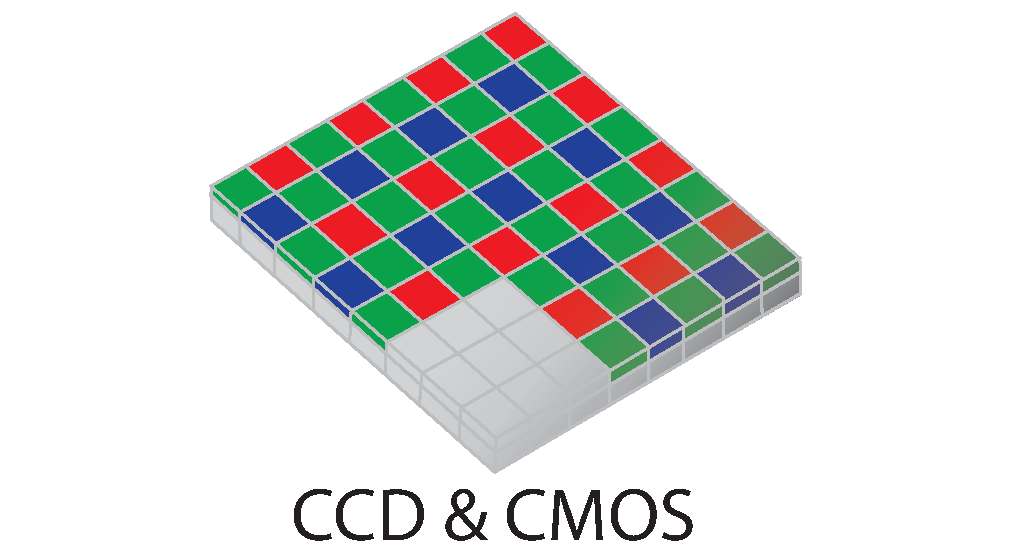
\includegraphics[width=70mm]{figures/CCDandCMOS.pdf}
\caption{Bayer filter}
\label{fig:example}
\end{figure}

What limit us to only use three spectral channels in image analysis is conventional thinking and that there are many cost effective camera in this range. When we register more than one spectral channel we need to use multiplexing, switching between channels either spatially or temporally. Ultimately it should be the application that decides how wide the spectral range should be and the number of channels. It is possible to achieve spectral imaging in a method similar to the Bayer filter, there are cameras with 9 (3 $\times$3) visible light channels and 16 (4 $\times$4) infrared channels that together can give us 25 channels simultaneously. As the number of channels increase to several hundred we call it \textbf{imaging spectroscopy} or hyperspectral imaging. This type of imaging creates a large amount of data and needs effective transmission and compression. 

A solution to capture a large number of spectral channels is to have a rotating filter wheel in front of a wide band, single channel sensor/sensing chip. This requires the scene to be stationary since there will be several images registered.

\subsection*{Temporal aspects (\textbf{t})}
Each image will register something for defined time interval and if there is only one single temporal slice we have a still image, while if there are multiple exposures we get a film/movie. For each captured image or exposure we need to define the exposure time, the following questions should be considered:

\begin{itemize}
	\item Does it give motion blur, how fast is the scene/object moving?
	\item Can it be varied freely?
	\item How will the quality of the image be affected by the exposure time? high ISO sensitivity more noise for example. 
\end{itemize}

During the exposure is each pixel, line or image exposed for a certain time, so we need to consider the motion in the scene and of the camera relative to it and the light intensity can by limited. There are however ways to freeze a moving object in the image by using a flash or follow the object in motion with the camera. There are even special solutions with sensors that have electronic object following. 

Using sequences of images can be useful when measuring a motion. It is then crucial with timing:
\begin{itemize}
 	\item Repetition time
 	\item Exposure time
 	\item Data transfer and storage time
 	\item Influenced by resolution in all five dimensions. 
 \end{itemize} 
Sequences can also be used to detect changes in scenes by subtracting the previous stored reference image. For a sequence to be perceived as continuous by the human visual system it is necessary to have a repetition frequency of at least 25 Hz.

Multiplexing is needed since the intensity must be measured for all pixels to get a complete image matrix and we have multiple spectral channels (color RGB) to consider in the integration process. There are no effective sensors that can capture all dimension at once and we need to multiplex the light collection. The amount of parallelism in this light collection is an aspect imaging system and is strongly influenced by how the light is handled (economically) by the system. 

\subsection*{Area integration}
Area integration in imaging technology that uses a 2D image sensor to register the light for the whole image in parallel is by far the most common. It started of with image tubes and was later replaced with \textbf{CCD} (Charge Coupled Device) that are now being replaced with \textbf{CMOS} (Complementary Metal Oxide Semiconductor) that could be replaced by new technologies like QIS (photon counting devices) in the future. 

Area integrations gives the best light collection efficiency since it collects "all the light". It also have a rigid geometry and gives stable and predictable imaging geometry that don't suffers from a lot of distortions. There is no need for mechanical motions and they can be mass-produced and therefore inexpensive. The drawbacks with area integration is that it need an even illumination of the whole image surface and there may be varying sensor sensitivities that need to be corrected for. It is also difficult to achieve high fill factor since there are other things that competes for space on the 2D area, multispectral scanning can therefore also be hard to achieve. The image size will be limited by the sensor size. 

CMOS and CCD matrices/sensors are available in many different version with a variety of megapixel resolutions for special applications. In some applications they can be cooled to very low temperatures that allows for long integration times when the light levels are very low. In contrast they can also be used to capture fast events like laser flashes. 

\subsection*{Linewise integration}
This kind of sensors are often find in scanners and can be moved to capture an image of the object, or the object can be moved over the sensor. It is also common in remote sensing like satellites that move along the earth surface. 

The technical advantages with line integrations are much better pointwise integration but worse economy compered to area. In motion the orthogonal line will be "frozen" which can be useful in some applications. It allows the use of the other dimension in a 2D sensor for the wavelength, for RGB and hyper spectral scanners \textcolor{red}{? read more}. It possible to create whats called "intelligent sensors" by having a processor for each pixel. 
The disadvantages are similar to area integration, it needs an even illumination along the scan line, it needs corrections of sensor sensitivity along the line of pixels. The 1D fill factor is important but not often a problem \textcolor{red}{meaning?}. There is also a risk for x-y in-homogeneity because of the widely different methods of scanning.  

\subsection*{Point-wise integration}
With this methods we register light from one pixel at a time and it requires motion to create the image. Here we most distinguish between what is moving:
\begin{itemize}
	\item The illumination
	\item The sensor
	\item The object
\end{itemize}
The method is mainly used in stationary conditions such as microscopy or scanning film or paper/document. Examples of applications are Drum scanner which produces very high quality scans of document or film. Other applications:

\begin{itemize}
	\item Flying spot scanner
	\item Microscopy
	\begin{itemize}
		\item Fluorescens
		\item Confocal
		\item Multi-photon
		\item Moving stage
	\end{itemize}
\end{itemize}

Some of the advantages are that it gives maximal possibilities for optimization of the measurement of each pixel and that i can have optimized optical path and sensor. No differences between the sensor properties of the different pixel sensors, i.e. only one pixel. It also have the advantage of not having a limit to the image size. The disadvantages are that it uses the incoming light poorly and need some sort of complex mechanical system for scanning which also results in it being very slow compared to the other methods. 

\subsection*{Multiplexing for volume imaging}
A few words about multiplexing and volume imaging; It is possible to register single voxels, a line, a plane at a time, the whole volume in parallel. Collecting data in the Fourier domain or through other transforms can be done. Today most tomographic systems collect data from the whole volume or from multiple planes simultaneously which is fast and therefore saves time and signal economy. 

\subsection*{Wavefront imaging}
Is new form of imaging that have high information density. The Wavefront sensing measure the amplitude and phase of the incoming optical field simultaneously. It is still under development but show promising results. 

\subsection*{Stored intermediate analogue image}
This category is mainly of historic interest and a few example are listed here:

\begin{itemize}
	\item Photographic film
	\item Polaroids
	\item Magnetic tape 
	\item Semiconductor materials (image plates)
\end{itemize}





    \lesson{2}{tuesday 17 jan 2023 10:15}{Graphics programming}


\section{Graphics programming}
Typicalli deals with how to define 3d scene, with virtual camera, how to create a 2d projection of the 3d scene

\subsection*{Real time vs ofline}
real time used in games, scene must be updated 30-60 fps
speed > im quality, but today hardware can do pretty much both

offline is used for animatied movies and visual effects. not meant to be used interactivly 
rendering a single frame can take several hours 
image qualite > speed. Movie production uses clusters to calculate the renders in pareallell

\subsection*{how do we draw}
version 1
for every pixel on the screen query all objects to be drawn there is a outher loop - ray tracing


version 2
iterate over objects
for every object draw the objects to the screen- rasterization
dont need to keep the whole scen in memory

\subsection*{Representation}

typically used for represent 3d models, vertices, edges and faces. faces can be arbritary polygons. Why do we split them in triangels? The implementation gets simpler 

\subsection*{vertex data}
polygonal mesh has one or several attributes 

\begin{itemize}
	\item Position
	\item Color
	\item Normal vector
	\item texture coordinate
\end{itemize}

vertex data is loaded on the cpu uploaded to the gpu \textcolor{red}{correct}

\subsection*{transform}
Use transforms to maniuplate positions orentation
use transforms to define our virtual camera
basic transforms:

\begin{itemize}
	\item scale ... \textcolor{red}{cont..} 
\end{itemize}


\subsection*{Cooerdinate systms}

THe OpenGL pipeline has 6 differnte systems

\begin{itemize}
	\item Object 
	\item World
	\item Eye (or camera)
	\item Clip
	\item Nomalized devices
	\item Window (or screen)
\end{itemize}

\subsection*{Surface normals}
a normal vector that points outwards from the surface..
descrives a local orientation. super important to lighting. Useful to know if the surface is pointing towards me or not 

Can visualize it with RGB vector for example.

\subsection*{Shaderds}
shader is a small program that is commpiled on the cpu and exectuted on the GPU. Common use is to apply fransfromations on vertices and compute 
\textcolor{red}{cont..} 

\subsection*{pipeline}
vertives -> sent to gpu -> assign attributes -> sent to clipper (remove what is not seen) and primitive assembler (takes vertices and conncect them to triangles) -> rasterized (converted into pixels or fragments) -> fragmen shader

We have controll of the vertices and the fragment shader from the cpu

\subsection*{OpenGL}

statebased maintain a currents state of things. what shader is being used etc. 
openGL for desktop
openGL ES for embedded
WebGl for 

it is a state machine

\subsection*{OpenGL functions}
executed in the host CPU application. It is responsible for creating and init buffers, shaders, tecture etc. 
uploading data to gpu 

\subsection*{The CPU and GPU}

\begin{wbox}{Simplified algorithm "immediate mode"}
init_system();
for (each object to be drawn)
	o = generate_object();
	draw_object

clean_up()
\end{wbox}

\begin{wbox}{Simplified algorithm v2}
init_system();
for (each object to be drawn)
	o = generate_object();

send objects to GPU
draw_all_objects()
clean_up()
\end{wbox}

sending objects complicated can become the bottleneck between the cpu and gpu


\subsection*{utility libraries}

glfw create and manage window
glew extension loader
glm mathematics library
imgui GUI

\subsection*{GLFW}
Give a interface between the windowing system and graphics system
allow us to create a window, ecectue tendering loop
cont..

\subsection*{GLEW}
cross platform search for extensions

\subsection*{GLM}
vector matrix datatypes  got a similar syntax as GLSL. Used in the hos 

\subsection*{ImGui}
Gui library for tweaking th e renderiung parameters
uses OoenGL so easy to implement 

\subsection*{RenderDoc}
can be useful in the project. hard to debug otherwise


\section{OpenGL}
\subsection*{vertex buffer}








    \section{Light microscopy}
Introduction to light microscopy. This chapter will cover: simple and compound microscopes. The general concepts of 
\begin{itemize}
	\item resolution
	\item magnification
	\item staining
\end{itemize}
It will also cover: Darkfield, phase contrast, Fluorescence and confocal microscopy.

	\subsection*{History}
	The father of microscopy: van Leeuwenhoek, he studied Hooke and refined his lenses to create a 1-lens microscope with approximately 270 times magnification. He used this to study insects, blood cells and bacteria. 


	\subsection*{Simple microscopes/magnifying glass}
	These types consist of one convex lens that enlarges the object. The magnification can be calculated with: $M = 1 + D/F$, where D is the least distance of distinct vision and F is the focal length of the convex lens. The maximum magnification that can be achieved this way is 10x. 

	\subsection*{Compound microscope}
	This type of microscopes are often referred to as \textbf{brightfield} microscopes. The concept: light from the light source is focused by a condenser onto the target/specimen. The transmitted light is then collected by the objective and forms a magnified, primary image. The primary image is magnified another time by the ocular lens. The total magnification of a compound microscope is given by the magnification of the ocular lens times the magnification of the objective lens. 

		\subsubsection*{Parts of a (typical) compound microscope}
		Light from the light source/illuminator goes through the condenser lens which focuses all the rays of light onto the specimen to maximize the illumination of it. By opening and closing the \textbf{diaphragm} between the condenser and the specimen it possible to adjust the amount of the light hitting the specimen. It is also possible to control the brightness of the light source with a \textbf{rheostat}. The light that hits the specimen is then differentially transmitted, absorbed, reflected or refracted by the different structures in the specimen. The \textbf{objective lens} collects the light and creates the magnified image which is magnified once again by the \textbf{ocular}. 

	\subsection*{The total magnification}
	The total magnification of the compound microscope can be expressed: M$_o \times$ M$_e$, or alternatively :

		\begin{equation}
		 	m = \frac{D} {f_0} \times \frac{L} {f_e} 
		 \end{equation}
	Where D is the least distance of distinct vision (25 cm), L the  length of the microscope tube, f$_o$ focal length of the objective lens and f$_e$ the focal length of the eyepiece/ocular. 

	It is the light and optics that define the possible resolution, expressed:

		\begin{equation}
			d = \frac{\lambda} {2n\sin\theta} 
		\end{equation}

	Where d is the \textbf{point resolution} (the short the better for us), $\lambda$ which is the \textbf{wavelength}, n the \textbf{refractive index} (1 for air, 1.3 for water or 1.4-1.5 for oil). nsin$\theta$ is the \textbf{numerical aperture}. 

	\subsection*{Numerical aperture}
	The numerical aperture defined as: NA = $n\sin\theta$ where n is the refractive index for the medium between the specimen and the objective. The angle $\theta$ is the angle of the light cone. A high NA means that the objective collects light efficiently, means that $\theta$ is large. A high NA also means high resolution. 

	\subsection*{Resolution}
	Resolution, the smallest features that can  be distinguished in the system. In a typical microcscope the resolution is decided by the wavelength of the light $\lambda$ and the \textbf{resolving power} of the microscopes objective, which is defined by its numerical aperture NA. 
	Somethings to consider: the maximum NA for an objective in air is 1. The resolution limit is given by the \textbf{Rayleight criterion}:

		\begin{equation}
		r = 0.61 \times \frac{\lambda} {NA} 
		\end{equation}

	An example using a wavelength of 550nm and objective with a NA of 0.7 gives a limit of 480nm. A cell is in the size of 10-30 $\mu$m and can therefore be observed in a light microscope. Viruses are on the other hand even smaller, $\approx$ 10-200nm and cannot be resolved by a ordinary light microscope. 

	With oil immersion its possible to increase the magnifications. This is possible thanks to the refractive index of oil is higher than air and similar to the glass that the specimen sits on. More light can be collected this way. 

	\begin{wbox}{Remember}
		  \textbf{Magnification without resolution is useless: empty magnification}
	\end{wbox}
	
	\subsection*{Airy disc}
	An Airy disc is the optimally focused point of light that can be determined by a circular aperture in the case of a perfectly aligned system limited by diffraction. If we view this from above it appears as a bright point with ripples around, also know as the airy pattern. The diffraction pattern is determined by the wavelength of light and the size of the aperture which the light passes through. The way a system images a point is called the \textbf{point spread function} or PSF for short. 

	\subsection*{Staining}
	Staining the sample is done to create contrast and or highlight details of interest. One very common stain is \textbf{H\&E - Haematoxylin and eosin} 

	\subsection*{Immunostaining}
	With this type of staining are primary antibodies used that can bind to specific targets. There is also often a secondary antibodies that bind to the primary ones. The secondary antibodies have a dye or fluorescence attached to them or an enzyme that induces a coloring reaction. 

	DAB staining is a derivative of benzene and most often used in immunohistrochemical staining as a chromogen (a colorless chemical compound that can by reaction turned into colored). In DAB staining is DAB oxidized by hydrogen peroxide in a reaction typically catalyzed by HRP. The DAB forms a brown preciptate \textcolor{red}{?} at the locations of the HRP, this can be visualized by a light microscope. 

	\subsection*{Typical immunohistochemistry staining procedure}
	Step by step:
	\begin{enumerate}
		\item Endogenous peroxidase are inactivated with hydrogen peroxide
		\item Then are the antigen exposed with HIER (heat induced antigen retrieval)
		\item Non-specific bindings sites and Fc repecptors get blocked by a normal serum (goat serum)
		\item The primary antibodies are applied and bind to the exposed antigen in the cells and cannot bind to any of the blocked ones. 
		\item Then is the secondary antibody applied which got peroxide polymer attached bind to the primary antibodies. 
		\item In the last step are the peroxidase developed with DAB and hydrogen peroxide which gives dark brown deposits at the site of the bound antibody.
	\end{enumerate}

	\subsection*{Possible issues - immunolabeling}
	
	\begin{itemize}
		\item High background
		\begin{itemize}
			\item Unspecific binding
			\item Endogenous peroxidase
			\item Excess peroxidase not washed away
		\end{itemize}
		\item Weak signal
		\begin{itemize}
			\item Not exposed antigen
			\item Not good antibodies
			\item Not enough time for reaction
		\end{itemize}
	\end{itemize}
	
	Useful to compare the result with correct negatives, correct positive and false positive references. Other sources of errors can be that the sample is old, the chemical / solutions are old or wrong protocol is followed \textcolor{red}{?}. 

	\subsection*{Dark field microscopy}
	 Microscopy in which the central part of the light cone from the source is \textbf{blocked}, the only light that reaches the objective is light that has been refracted or reflected by the structures in the specimen (scattered light ?). This means that \textbf{no direct} light from the condenser enters the objective lens. The result has good contrast and resolution without any staining. This means that the technique is good for live specimens that otherwise would have been killed by the stains.  

	 \subsection*{Phase contrast microscopy}
	 Invented by Fritz Zernike in 1941. Uses the property that light phase shift when passing through a transparent specimen, different refractive index of different constituents turn into amplitude changes that creates the contrast in the image. This technique doesn't need any stain, no fixation, and is good for live cells. Good option for imaging objects with no color. 

	 \subsection*{Differential interference contrast microscopy}
	 Invented in the early 50's. It is a technique with good contrast without staining, for transparent objects for an example. It uses polarized light and interferometry. The contrast is created due to the differences in path length for two adjacent points in the sample. It can image small differences in the refractive index between neighboring points.

	 \subsection*{Reflected light microscopy}
	 Also known as episcopic illumination metallography microscopy. Typically used for imaging the surface of metals, plastic, ores, ceramics, paper and so on. Same principle as but here are mirrors used to reflect the light onto the object. 

	 \subsection*{Confocal microscopy}
	 First patented in 1957. The method was improved with laser technology and became generally accepted and a very popular technique. A confocal microscope focus on one point at a time and can scan across the specimen in x,y \textbf{and} z direction. The results are 2D images at various depths which can be reconstructed / stacked to form a 3D image. Flourescent stain are often used to increase the contrast and resolution. The image clarity and resolution is improved by a narrow aperture that eliminates light that is not from the z-plane. This technique is useful for examining thick specimens and can also be used on live, unfixed samples. 

	 \subsection*{Fluorescence microscopy}
	 A technique that uses fluorescent molecules \textbf{fluorochromes} or \textbf{fluorophores} that absorb energy from a light source and emits the energy as light of a different wavelength. There are natural fluorecents (chlorophylls) and fluorescent stains that are added to the specimen to create contrast for the image.

	 The principle behind fluorescent microscopy: 

	 \begin{itemize}
	 	\item High energy light source emit light 
	 	\item An excitation filter decides what wavelength to let through to illuminate specimen
	 	\item The fluorophores in the specimen absorb the energy from the light and emit energy with a longe wavelength. 
	 	\item A dichroic mirror reflect the light of the excitation wavelength and tramsit light of the emission wavelength, so only the light of interest passes.
	 	\item This mirror is not perfect so not all light is blocked. 
	 \end{itemize}

	 \subsection*{Fluorophores}
	 In microscopy are most fluorophores excited near UV,blue or green light. A mercury arc lamp is an ideal light source that provide high intensity in the wavelength : 365, 405, 436 and 646 nm. 

	 \subsection*{Stoke shift}
	 The stoke shift is the energy difference between the peak of absorbance and the peak of the highest emission energy. Without the stoke shift it wouldn't be almost no way of distinguish between excitation and emitted light. Probes\textcolor{red}{(?)} with varying Stoke shift are useful for multicolor applications. 

	 \subsection*{Autofluorescence}
	 Autofluorescence is the natural emission of light by biological structures such as mitochondria and lysosomes after they absorbed light. This is then used to distinguish the light from the artificially added fluorescent markers (fluorophores). \textcolor{red}{?} 

	\subsection*{green fluorescent protein}
	Green fluorescent protein also know as GFP exhibits green fluorescence when it is exposed to light in the UV range. GFP was first isolated from a jellyfish. This GFP has a major excitation peak at 395nm and a minor one at 475nm while the emission peaks at 509nm. This GFP gene is frequently used as a reporter of expression \textcolor{red}{?}. The gene is inserted together with the gene of interest and if the GPF is expressed then we can assume the  gene of interest is that also.

	\subsection*{Immunofluorescence}
	Fluoochrome attached to primary or secondary antibodies can be used to visualize the location of targets. This is used a lot in cell biology. 

	\subsection*{2- or multi-photon microscopy}
	here the fluorophore is excited with 2 or more photons of lower energy (if two half excitation), hitting it simultaneously. One can use pulsed lasers for this and there is no need for pinhole since the emission will only happen from the focus spot. The advantage of this technique are the reduced phototoxicity and increased image depth. 
	 





    %!TEX root = master.tex


    \section{Model-free control}
Model-free control is a class of algorithms that aim to learn an optimal policy directly from interacting with the environment without building an explicit model of the environments dynamics. They rely on a trial and error experience to update the estimate of the value-functions or action-value functions. Examples are Q-learning, learning the Q-function and SARSA learning the value-function. 

\subsection*{Model free control}
How do we improve the policy? One way is to take the greedy policy improvement with respect to the state value-function $v_\pi(s)$:
	
	\begin{equation}
		\pi^{\prime}(s) = \underset{a}{\arg \text{max }} \sum_{s^{\prime}, r}^{}p(s^{\prime},r |s,a)[r+\gamma v_\pi(s^{\prime})]
	\end{equation}

But this requires us to know the model: $p(s^{\prime},r|s,a)$. If we instead take the greedy policy improvement with respect to the action value function we got:

	\begin{equation}
		\pi^{\prime}(s) = \underset{a}{\arg \text{max }} q_\pi(s,a) 
	\end{equation}

In this case we don't need the model. So the first idea is to estimate the action-value function $q_\pi(s,a)$ instead of the state value-function $v_\pi(s)$

\begin{example}{Example: Can we learn enough from greedy actions}
\begin{itemize}
	\item \textbf{Initial: } Q(left) = Q(right) = 0
	\item You open left and get the reward 2:
		\begin{equation*}
			\text{Q(left) =2, \text{Q(right)=0}}
		\end{equation*}
	\item You open left and get reward 0:
		\begin{equation*}
			\text{Q(left) =1, \text{Q(right)=0}}
		\end{equation*}
	\item You open left and get reward 4:
		\begin{equation*}
			\text{Q(left) =3, \text{Q(right)=0}}
		\end{equation*}
\end{itemize}

With this approach we will never learn about what happens if we would open the right door
\end{example}	

With that example in mind we present idea 2: make sure that we continue to explore different options!

\subsection*{$\epsilon$-greedy exploration}
There is a trade-off between exploiting current knowledge and exploring new options. A possible solution is to ensure that all actions have non-zero probability. We call this policy $\epsilon$-greedy policy: If $\pi (a|s) \ge \frac{\epsilon} {|\mathcal{A}|} $ for all $a$ and $s$. 

\begin{itemize}
	\item $\epsilon$-greedy with respect to $q_\pi(s,a)$: 
	\begin{itemize}
		\item with probability 1 - $\epsilon$ choose a greedy action $\underset{a}{\arg \text{max }} q_\pi(s,a)$
		\item with probability $\epsilon$ choose an action at random.
	\end{itemize}
\end{itemize}

\begin{wbox}{Policy improvement theorem}
For any $\epsilon$-soft policy $\pi$, the $\epsilon$-greedy policy $\pi^{\prime}$ with respect to $q_\pi$ is an improvement, i.e.

	\begin{equation}
		v_{\pi^{\prime}}(s) \ge v_\pi(s), \quad \text{for all } s \in \mathcal{S}
	\end{equation}
\end{wbox}

The conclusion is that: policy improvement with $\epsilon$ policies will converge to the best $\epsilon$-soft policy. 

\subsection*{On-policy vs off-policy learning}
With in-policy learning we can say that we are "learning on the job" by estimating the action value function $q_\pi(s,a)$ by running the policy $\pi$. In off-policy learning we "learn by looking over the shoulder", estimate the action value-function $q_\pi(s,a)$ while running a different policy $\mu$. For example we learn about $q_*(s,a)$ (optimal q-function), while running a policy with more exploration.


\subsection*{Monte-Carlo control}
We use the policy to collect trajectories: $S_0,A_0,R_1,S_1,A_1,R_2,\ldots,S_T$. Then estimating the state-value function by computing the average over all returns seen from each state. The incremental update is:

	\begin{equation}
		V(S_t) \leftarrow V(S_t) + \alpha(G_t - V(S_t))
	\end{equation}

For estimating action-value function we compute the average over all returns seen from each state/action-pairs and the incremental update is:

	\begin{equation}
		Q(S_t,A_t) \leftarrow Q(S_t,A_t) + \alpha(G_t - Q(S_t,A_t))
	\end{equation}

\subsection*{Exploration is needed!}
The estimation of the state-values: $V(S_t) \leftarrow V(S_t) + \frac{1} {N(S_t)}(G_t - V(S_t))$, converges to $v_\pi(s)$ as $N(s) \rightarrow \infty$ \\
Estimation of action-values: $Q(S_t,A_t) \leftarrow Q(S_t,A_t) + \frac{1} {N(S_t,A_t)}(G_t - Q(S_t,A_t)) $, converges to $q_\pi(s,a)$ as $N(s,a) \rightarrow \infty$. However if the policy $\pi (s|a) = 0$ for some s and a then we will not learn this action-value! With a $\epsilon$-soft policies we guarantee that $pi (a|s) > 0$ for all s and a.

As long as we use a $\epsilon$-soft policy $Q(s,a)$ will converge to $q_\pi(s,a)$ as the number of sampled episodes goes to $\infty$. Now it is time to improve the policy!!

\subsection*{Monte-Carlo policy iteration}
The policy evaluation: Monte-Carlo evaluation is used to get $Q = q_\pi$. The policy improvement: we let a new policy $\pi$ be $\epsilon$-greedy with respect to $q_\pi$. This will converge to the best $\epsilon$-soft policy. For this we need infinitely many episodes to guarantee that $Q = q_\pi$ which is not possible in practice. 

\begin{itemize}
	\item At every episode:
	\begin{itemize}
		\item Policy evaluation: Use MC to update Q.
		\item Policy improvement: Let new $\pi$ be $\epsilon$-greedy with respect to Q.
		\item On policy: we always update Q toward $q_\pi$ for the the current policy.
	\end{itemize}
\end{itemize}

\begin{wbox}{Monte-Carlo control}
	\begin{enumerate}
		\item Initialize Q (in other words Q(s,a) = 0 for all s and a) and let $\pi P \epsilon$-greedy(Q)
		\item Sample episode using $\pi: S_0,A_0,R_1,\ldots,S_T$
		\item For each state $S_t$ and action $A_t$ in the episode:
			\begin{equation}
			\begin{aligned}
				N(S_t,A_t) \leftarrow N(S_t,A_t)+1 \\
				Q(S_t,A_t) \leftarrow Q(S_t,A_t) + \frac{1} {N(S_t,A_t)}(G_t - Q(S_t,A_t)) 
			\end{aligned}
			\end{equation}
		\item Improve policy: $\pi \leftarrow \epsilon$-greedy(Q)
		\item Go to step 2 
	\end{enumerate}
\end{wbox}

\subsection*{Exploration}
If we converge we get the best policy among the $\epsilon$-soft policies. It is possible to gradually reduce the $\epsilon$ (but not to fast) toward zero, in order to converge to the optimal policy. Then after training we can remove the exploration by setting the $\epsilon = 0$ and thus using the greedy policy with respect to Q. 

\subsection*{SARSA}
If we return to MC and TD (aka SARSA) and compare these. TD has several advantages over MC-prediction: Lower variance, the capability to run online, without waiting to end of episode and it can be used with incomplete sequences. SARSA can apply TD to $q_\pi(s,a)$ and use $\epsilon$-greedy policy improvements, and improve every time-step. 

	\begin{equation}
	\begin{aligned}
		 		v_\pi(s) = \mathbb{E}_\pi[R_{t+1} + \gamma v_\pi(S_{t+1})|S_t =s] \\
		 		q_\pi(s,a) = \mathbb{E}_\pi[R_{t+1}+ \gamma q_\pi(S_{t+1}, A_{t+1}) | S_t = s, A_t = a]
	\end{aligned}
	\end{equation}

Estimating the state-values with given $\{ S_t, R_{t+1},S_{t+1}\} \sim \pi$ the update is:

	\begin{equation}
		V(S_t) \leftarrow V(S_t) + \alpha (\underset{\text{Target}}{R_{t+1}+\gamma V(S_{t+1}) }- V(S_t))  
	\end{equation}  

Estimating the action-values with SARSA given $\{S_t,A_t,R_{t+1},S_{t+1},A_{t+1}\} \sim \pi$ the update will be:

	\begin{equation}
		Q(S_t,A_t) \leftarrow Q(S_t,A_t) + \alpha (\underset{\text{Target}}{R_{t+1} + \gamma Q(S_{t+1},A_{t+1})}-Q(S_t,A_t))
	\end{equation}

\subsection*{SARSA control}

\begin{itemize}
	\item At every time-step:
	\begin{itemize}
	\item \textbf{Policy evaluation: } Use SARSA to update Q
	\item \textbf{POlicy improvement: } Let new $\pi$ be $\epsilon$-greedy with respect to Q
	\item \textbf{On-policy: } We always update Q towards $q_\pi$ for current policy
\end{itemize}
\end{itemize}


\begin{wbox}{SARSA-algorithm for control}
\begin{itemize}
	\item Initialize Q(s,a) in other words Q(s,a) = 0 for all s and a.
	\item For each episode
		\begin{enumerate}
			\item Get initial state S
			\item Choose A from S that is $\epsilon$-greedy with respect to Q
			\item For each step of episode:
			\begin{itemize}
				\item Take action A and observe $R,S^{\prime}$
				\item Choose $A^{\prime}$ from $S^{\prime}$ that is $\epsilon$-greedy with respect to Q
				\item $Q(S,A) \leftarrow Q(S,A) + \alpha (R + \gamma Q(S^{\prime}, A^{\prime}) - Q(S,A)) $
				\item $S \leftarrow S^{\prime}, A \leftarrow A^{\prime} $
			\end{itemize}
		\end{enumerate}
\end{itemize}
\end{wbox}

\subsection*{Off-policy control - $\mathcal{Q}$-learning}
Here the goal is the learn the action-value function $q_\pi(s,a)$ for a target policy $\pi$ with experience from using the \textbf{behavior policy} $\mu$. This is useful when we want to learn by observing how humans or other agents act. It is also useful when we want to re-use experience that is already collected from old policies. It is also useful when we want to learn the optimal $q_*(s,a)$ while following an exploratory policy.

	\begin{equation}
	 	q_\pi(s,a) = \mathbb{E}_\pi \left[ R_{t+1} + \gamma q_\pi(S_{t+1}, \underset{\sim \pi (a|S_{t+1})}{A_{t+1}}) | S_t=s, A_t = a \right]
	 \end{equation} 

If we consider the data collect using the behavior policy $\mu$ 

	\begin{equation}
		S_t,A_t,R_{t+1},S_{t+1},A_{t+1} \sim \mu
	\end{equation}

Then update: let $A^{\prime} \sim \pi (a|S_{t+1})$ and use the update:

	\begin{equation}
		Q(S_t,A_t) \leftarrow Q(S_t,A_t) + \gamma(R_{t+1} + \gamma Q(S_{t+1},A^{\prime})-Q(S_t,A_t))
	\end{equation}

We want both behavior and target policies to improve. The \textbf{target policy}, $\pi$: Greedy with respect to Q(s,a) and \textbf{behavior policy, }$\mu$: $\epsilon$-greedy with respect to Q(s,a). The Q-learning target is then:

	\begin{equation}
 		R_{t+1} + \gamma Q(S_{t+1},a)
 	\end{equation}

Here is $A^{\prime} = \underset{a}{\arg \text{max }}Q(S_{t+1},a)$. If we insert this we can rewrite the target as:

	\begin{equation}
	\begin{aligned}
		R_{t+1} = \gamma Q(S_{t+1}, \underset{a}{\arg \text{max }} q_*(S_{t+1},a)) = \\
		R_{t+1} + \gamma \underset{a}{\text{max }}q_*(S_{t+1},a)
	\end{aligned}
	\end{equation}

We can compare this to the Bellman optimality equation:

	\begin{equation}
		q_*(s,a) = \mathbb{E}[R_{t+1} + \gamma \underset{a}{\text{max }}q_*(S_{t+1},a)|S_t=s,A_t =A]
	\end{equation}

\begin{wbox}{The Q-learning theorem}
Q-learning converges to the optimal action-value function $q_*(s,a)$ as $N(s,a) \rightarrow \infty$ if the step size $\alpha$ decreases toward 0 with a suitable rate.  
\end{wbox}




























    \section{Ultrasound}
Ultrasound (and all other types of sounds) are acoustic waves, i.e. a mechanical perturbation traveling in a medium. The acoustic frequency range:

\begin{itemize}
	\item Infrasound: < 20 Hz
	\item Audible sound: 20 Hz - 20 kHz
	\item Ultrasound: > 20 kHz 
	\item (Medical ultrasound: 1 - 20 MHz) 
\end{itemize}

Ultrasound is therefore mechanical oscillations with a frequency above 20 kHz that propagates through a medium that is elastic. Used for finding fungus in trees, used by bats to find their prey and in quality control of weld joint for finding cracks to give a few examples. The discovery of the piezoelectric property made this technique possible. 

	\subsection*{Ultrasound in medical imaging}
	Ultrasound is one of the most used imaging techniques in medicine and have an annual market growth of 3-4\%.Pros for this technique are that is non ionizing, need minimal safety requirements, its real time, can be made portable and is quite low cost. The downside with real time is the need of training personnel to understand/interpret the image while making the examination. Signal to noise ratio is quite low compared to other techniques and it need a acoustic window to operate (can't "see through" bone). 

	\subsection*{Probe - probing mechanism}
	Ultrasound is a longitudinal wave, variation of pressure that propagates, this mean that it needs a medium to travel through. The speed of sound is a function of the medium:

		\begin{equation}
			c = \sqrt{\frac{K} {\rho} }		
		\end{equation}

	Where K is the stiffness, stiffer the faster and $\rho$ is density: denser the slower. Like electrical circuits with resistance and current, the propagation of sound can be calculated with the Acoustic impedance:

		\begin{equation}
			Z = \rho c
		\end{equation}

\newpage

		\begin{table}[ht!]
		\centering
		\begin{tabular}{lllm{5cm}}\hline
		\textbf{Material} & bf\textbf{Density (kg$\text{m}^{-3}$)}& \textbf{Speed of sound}& \textbf{Acoustic impedance \newline (kg$\text{m}^{-2}$$\text{s}^{-1} \times 10^6$ )} \\

		Air & 1.3 &  330& 0.000429\\

		Water & 1000 & 1450& 1.50\\

		Bone & 1500 & 4000& 6.0\\
		
		Blood & 1060 & 1570& 1.59\\

		Muscle (average) & 1075 & 1590& 1.70 \\ \hline
		
		\end{tabular}
		\caption{Example of a table with line breaks}
		\label{tab:example}
		\end{table}

	The \textbf{wavelength} $\begin{bmatrix} m \end{bmatrix}$ is determined by: \textbf{Frequency} $\begin{bmatrix} Hz \end{bmatrix}$ (depends on the source) and \textbf{Sound-speed} $\begin{bmatrix} m/s \end{bmatrix}$ (depends on medium). 

	\subsection*{Matter interaction}
	After the sound wave left the source (probe) it interact with the material with the tissue, being \textbf{back-scattered}, \textbf{reflected}  and \textbf{refracted}. The sound wave is attenuated while moving through the tissue. 

	When the wave travels into a new medium the impedance of the medium and the incidence angle determines what happens to the wave (Huygens principle). If the wavefront is perpendicular to the medium the wavelength will change. If there is an oblique incidence angle it \textbf{refracts} giving a \textbf{reflection} against the new medium and \textbf{transmitted} wave through the new medium. The intensity of each part is dependent on: the \textbf{acoustic impedance difference} between the two materials and the \textbf{angle of incidence}.

	\textbf{Scattering} is the directionless reemission of incident energy caused by local inhomogeneities. Inside tissue, this scattering is caused by "tiny" particles, cells, large proteins, calcifications and so on. The interaction between this scattered waves is what causes the noisy speckle texture pattern in ultrasound images. 

	\textbf{Attenuation} is the loss of energy of the wave in the material. This energy is lost over distance due to \textbf{absorption}, \textbf{scattering}, mode conversions \textcolor{red}{?} and more. The amplitude decay increases with the depth (z) as a function of \textbf{some tissue properties} ($a_0$) and \textbf{acoustic frequency)}(f) 


		\begin{equation}
		A(z) = A_0 e^{-a_0 f^{n}z}
		\end{equation}

		\begin{wbox}{The tradeoff}
			\textcolor{OliveGreen}{The higher the frequency, the better the imaging resolution } \\
			\textcolor{red}{But, the worse the penetration depth} 
		\end{wbox}
	
	\subsection*{Piezo-electric effect}
	The purpose of the ultrasound transducer is to convert between electrical signal and acoustic energy. It act as both speaker and a microphone. By first emitting a very short sound pulse and then listen to the returning echoes (for a longer time then the emitting time). It is only possible to to one at a time. 

	The piezo-electric effect is a property that certain solids can have (some crystals and ceramics). Expose the material for electricity and there will respond with mechanical stress (like a speaker). Swapping places and expose it for mechanical stress will produce an electrical current (like a microphone)

	\subsection*{Image production}
	Producing the image involves switching between Transmit (Tx) mode : active (speaker) and Receive (Rx) mode : passive (microphone). There are different modes for the imaging also:

		\begin{itemize}
			\item \textbf{A(mplitude)-mode:} one scan line
			\item \textbf{B(rightness)-mode:} 2D spatial images with multiple neighboring A-lines
			\item \textbf{M(otion)-mode:} sequences of A-modes in time, thus 2D (popular in cardiology) 
		\end{itemize}

	Beamforming is the technique used to form sensor arrays for directional transmission and reception. By adjusting a time delay between element it is possible to mimic the spatially focus of a curved transducer. 

	\textcolor{red}{insert US focus illustration here} 


	\subsection*{Image quality}
	Contrast is what assesses visibility, so by comparing the image appearance between two distinct regions we want to be able to distinguish between object and background. 


















	



    \section{PET, CT and MRI}
All of these techniques are so called tomography techniques (imaging slices of the sample). They are used in both clinical routine and in research. In common that they are: expensive, risks involved in using them (Radioactivity, Ionizing radiation and strong magnetic fields). The geometrical accuracy is good for all of them with some exceptions for MRI. Can perform both static and dynamic imaging (time series). They share the challenges of tunnel size (PET/MRI and MRI). Much development is ongoing, PET tracers, hardware and software. 

	\subsection{PET - Positron Emission Tomography}
	Uses a \textbf{tracer} or radio pharmaceutical that is emitting positrons. This radionuclide isotope is attached on a molecule of interest, glucose for an example in Fluorodeoxyglucose $^{18}F$. The doses are small (microdosing) and there is no expected pharmacological effect of the patient. The PET systems create an image of the concentration of tracer. There are many different types of tracers, and more under development. Depending on what is needed to be imaged or what is being looked for the tracer is chosen. The images are typically of quite low resolution and don't give much anatomical information, it is therefore most often combined with MRI or CT. 

		\subsubsection{Workflow}
		The unstable isotope is created in a cyclotron often close to the PET facility, since the halftime is often short. It is then combined with the molecule of interest and we have the tracer that can be injected into or in some cases inhaled by the patient. The tracer emits positrons (beta particles) that can only travel short distances (mm) before it annihilates with an electron and create two 2 gamma rays shooting of approx 180 degrees apart. The detector rings picks up these gamma rays (Coincidence detection) and counts them, giving a line of response (LoR). This results in a\textbf{Sinogram} that is reconstructed with reconstruction algorithms including corrections for \textbf{random counts, attenuation and scatter}. 

		\subsubsection{Use cases}
		PET scanning is used to diagnose cancer, dementia and cardiac problems. It is also used in drug development. Examples of some measurements are:

			\begin{itemize}
				\item Glucose metabolism
				\item Blood flow
				\item Heart function
				\item Bone formation
				\item Receptor expression \textcolor{red}{?} 
			\end{itemize}

		\subsubsection{Tracers and isotopes}
		There are many different types of tracers for different kind of research and diagnosis purposes. Here are some to mention a few: 
			\begin{itemize}
			 	\item $^{18}$F-FDG used in oncology and neurology
			 	\item PSMA (prostate cancer)
			 	\item FLT (cancer)
			 	\item PiB (Alzheimer's)
			 \end{itemize} 
		The isotopes commonly used and their \textbf{half time (min)}:
			\begin{itemize}
				\item $^{82}$Rb-Rubidium \textbf{1.3}
				\item $^{15}$O-Oxygen \textbf{2}
				\item $^{13}$N-Nitrogen \textbf{10}
				\item $^{11}$C-Carbon	\textbf{20}
			\end{itemize}
		
		\subsubsection{Scanning}
		Three modes of PET scanning: Static scans with about 20cm of coverage, Dynamic scans: time series of scans and Whole-body scans: combination of multiple 20cm scans. 

		\subsubsection{Reconstruction}
		Two types of image reconstruction: Filter back propagation which can be seen as fast and simple and Statistical likelihood-based which is iterative, uses more advanced modelling and corrections. The later one is therefore more computationally demanding. 
		Corrections for scatter and random coincidences are typically included.

			\begin{itemize}
			  	\item True Coincidence
			  	\begin{itemize}
			  		\item One annihilation
			  		\item Straight path of the photons in opposite direction 
			  	\end{itemize}
			  	\item Scatter coincidence
			  	\begin{itemize}
			  		\item One annihilation
			  		\item Photons scatter
			  		\item Measured line of response places annihilation reaction along artifact projection
			  	\end{itemize}
			  	\item Random coincidence
			  	\begin{itemize}
			  		\item More than one annihilation
			  		\item Photons from different annihilation detected at same time
			  		\item Artifact line of response 
			  	\end{itemize}
			  \end{itemize}  

	\subsection{CT - Computed Tomography}
	This technique uses X-rays that are sent through the body from different angles by rotating X-ray source and detector around the body. The X-rays are attenuated differently by different tissues and an image can be reconstructed from this "attenuation map". Arms up during the scan gives better image quality. It is a axial technique that is fast and high resolution. There are variations of it:
		\begin{itemize}
		  	\item High and low dose
		  	\item Contrast agents: intravenous or oral
		 \end{itemize}  
	Tissues have different attenuation, uses the Hounsfield scale. Calibrated with water = 0. 

		\begin{table}[ht!]
		\centering
		\begin{tabular}{ll}\hline
		 \textbf{Tissue}& \textbf{Hounsfield unit (HU)}   \\
		 Bone&    >400\\
		 Organs&   -30 +150\\
		 Water&    0\\
		 Fat&    -190 -30\\
		 Aire&    -1000\\ \hline
		\end{tabular}
		\caption{example}
		\label{tab:tab1}
		\end{table}

		\subsubsection{Use cases}
		CT scanning is used for diagnosis and follow up in \textbf{Cancer}, Acute medicine such as \textbf{trauma}, \textbf{strokes} and \textbf{hemorrhage}, \textbf{Surgery} (planning: inflammatory disease) and \textbf{Cardiac} function (requires fast machines).

		\subsubsection{Scanning}
		The scanning is always done in axial plane. The result is of high resolution Sinogram that needs reformatting afterwards. Alternatives are :
			\begin{itemize}
		 		\item Axial (can be preferred for brain scan)
		 		\item Spiral (Helical scan)
		 		\item Single or multi slice (16/64/128), multiple detectors instead of 1 long.
		 		\item Dual-energy CT
		 	\end{itemize} 		
		
		\subsubsection{Photon counting CT}
		There has recently been a major breakthrough in CT imaging thanks to photon counting sensors. These makes it possible to make smaller detector pixels that improves spatial resolution. \textcolor{red}{Intrinsic spectral sensitivity: multi energy information}, results in lower radiation exposure since there is lower electronic noise. Example of slice thickness: 0.2mm

	\subsection{MRI - Magnetic resonance imaging}
	Previously called: Nuclear Magnetic Resonance - NMR. The pros of MRI is the good soft tissue contrast, it uses no ionizing radiation and is very versatile: many different contrast mechanisms, used from morphology to physiology down to metabolism, can image angled slices. The Cons of the MRI systems are that they are: time consuming (examination time, patient motion problem), it is expensive, claustrophobia and competence need. 

		\subsubsection{What is imaged}
		The hydrogen "protons" have a property called \textbf{spin} that is used for the creation if the MR images. Spin is a quantum mechanical property, something that spins have angular momentum. Isotopes that have an odd number of protons or neutrons have a spin that is non zero. These can be studied by MR, they are usually : $^{1}$H or ($^{13}$C, $^{31}$P, $^{3}$H, $^{129}$Xe). Hydrogen is the most common atom in the human body with spin. 

		\subsubsection{Trade-off in MRI}
		To acquire an image with higher resolution means that it takes longer time if we want to maintain the same SNR, if we accept more noise we can do it with the same time. Since it can be required of the patient to hold their breath it might not be possible to change the time to much. 

		\textcolor{red}{trade-off triangle image}

		\subsubsection{General properties}
		The image elements are non-isotropic voxels and can be of the size: 1x1x6mm for an example. The intensities of the voxels are typically arbitrary units but can in some images be absolute. There are like in other imaging techniques artifacts. In MR there are often: intensity inhomogeneities, motion artifacts ans geometric distortions.

		
		\subsubsection{Spin, Precession, Larmor frequency}
		The hydrogen (proton) spin with a \textbf{Precession} (Like the earth has an angle in its rotation). This correspond to a frequency, the \textbf{Larmor frequency} which depends on the \textbf{B}$_0$ field: 64MHz at 1.5T and 128MHz at 3T. We can think of this "spin" as small magnets. Even though we apply a strong magnetic field, the net magnetization \textbf{M}$_0$ is very small, a few ppm compared to the unordered state without the magnetic field \textbf{B}$_0$ applied. Increasing \textbf{B}$_0$ increases the this magnetization \textbf{M}$_0$.

		\subsubsection{Excitation and relaxation}
		Hitting the spins with a radio wave with the \textbf{Larmor frequency} changes the net magnetezation into a state of \textbf{Excitation}, the spins precess in phase. Enter a state with \textbf{Longitudinal} and \textbf{Longitudinal}-magnetization (can detected). After that comes \textbf{Relaxation} where the "echo" is picked up by RF-antenna.

			\begin{wbox}{Image contrast}
				"When and how the MR signal is measured determines image contrast " \\
				"The whole process is repeated many times to collect the data needed"	
			\end{wbox}

		\subsubsection{T1 and T2 relaxation}
		The Longitudinal relaxation, when M$_z$ increases is called \textbf{T1} relaxation. The transverse relaxation, when M$_{XY}$ decreases is called \textbf{T2} relaxation. 

			\begin{itemize}
				\item Difference in \textbf{T1} relaxation between tissues determine the contrast in \textbf{T1-weighted} imaging
				\item Difference in \textbf{T2} relaxation between tissues determine the contrast in \textbf{T2-weighted} imaging
			\end{itemize}	
		
		\subsubsection{Repetition time (TR), Echo time (TE)}
		By changing the scanning parameters TR and TE the weighting of the contrast for different tissues changes. 

			\begin{table}[ht!]
			\centering
			\begin{tabular}{lll}\hline
			 \textbf{Weightings}&  \textbf{TE \& TR}&   \\
			 T2w& Long TE and long TR &  Long T2 gives strong/bright signal\\
			 T1w&  Short TE and short TR & Short T1 gives strong signal \\
			 PDw&  Short TE and long TR  & Many protons give strong signal\\ \hline
			\end{tabular}
			\caption{example}
			\label{tab:tab1}
			\end{table}

		\textcolor{red}{INSERT TR TE IMAGE} 
		
		\subsubsection{T1 and T2 in different tissues}
		T1 and T1 can be seen as tissue properties, but they are dependent on: disease conditions (which is good for diagnostic), contrast agents (that are used for changing relaxation times), the field strength and temperature.

		\subsubsection{Image generation (2D)}
		\textbf{Spatial encoding}is used to determine what slice is being image and to determine what is up/down and right/left in that slice. The principle for spatial encoding is \textbf{frequency encoding} which can be described like choir that sing brighter the further away they stand from the observer, from this we can determine position from the notes (in one direction at least). This principle is used by adding a linear magnetic field gradient (\textbf{G}) to the static magnetic field (\textbf{B}$_0$) in the scanner. By doing this, the total magnetic field and Larmor frequency will vary linearly with the position.
		\textbf{In-slice encoding} two directions are needed for encoding in the 2 dimensional slice, to do this simultaneously we use \textbf{phase encoding} also. The resulting signal readout repeated with different phase encoding results in a \textbf{k-space} image. Using the Fourier transform \textbf{FFT} we go from k-space to \textbf{image space}. To summarize: a combination of RF signals and a sequencing of linear gradients allow imaging.  
		
		\subsubsection{Image generation (3D)}
		Comparing 2D and 3D imaging:

			\begin{table}[ht!]
			\centering
			\begin{tabular}{ll}\hline
			 \textbf{2D}&   \textbf{3D} \\
			 Many slices to be excited to cover volume&  Two-phase encoding directions  \\
			 K-space in 2D& takes time, many TR's  \\
			 &  Short TR (and TE) needed \\
			 & Mostly for T1w   \\
			 & K-space in 3D \\
			 & Typically most time efficient for volume \\ \hline
			\end{tabular}
			\caption{example}
			\label{tab:tab1}
			\end{table}

		\textbf{Multi-slicing}, introducing the problem: A T2-weighted image used a long TR and TE, this means that there is a long waiting time to next excitation of the slice. This waiting time results in a lot of "deadtime" in the protocol. To be more effective was multi-slicing introduced. Additional slices are excited during the waiting time which means that the total scan time is reduced if TR increases (so that more slices fits under one TR).

		\subsubsection{Quantification of T1, T2 and PD}
		Instead of imaging with contrast weighting its possible to quantify the \textbf{relaxation parameters}. This is done by collecting data (multiple images) with different parameters, for example:

			\begin{itemize}
				\item For T2: different TEs
				\item For T1. different TRs 
			\end{itemize}

		 Then the signal \textbf{model} is fitted to the datapoints - voxel wise. This can be optimized in many ways, modelling and the data collection.  


		    
		

		          
		
		

		
			







	
    %!TEX root = master.tex

\section{Policy gradient methods}
Policy gradient methods are a class of model-free reinforcement learning algorithms that directly optimizes the policy, maps the states to action by using gradient descent. By using gradient of the expected return with respect to the policy parameters, these class of methods iteratively updates the policy to improve the performance. 

\subsection{Value-based vs Policy based RL}
The value-based RL methods are what we have looked at so far. Here we learn the value function and act greedily ($\epsilon$-greedy). In policy-based methods we don't use a value function, but learn a policy instead. In the next chapters we will take a look at Actor-critic methods were we learn the value function and policy.

\begin{figure}[ht!]
\centering
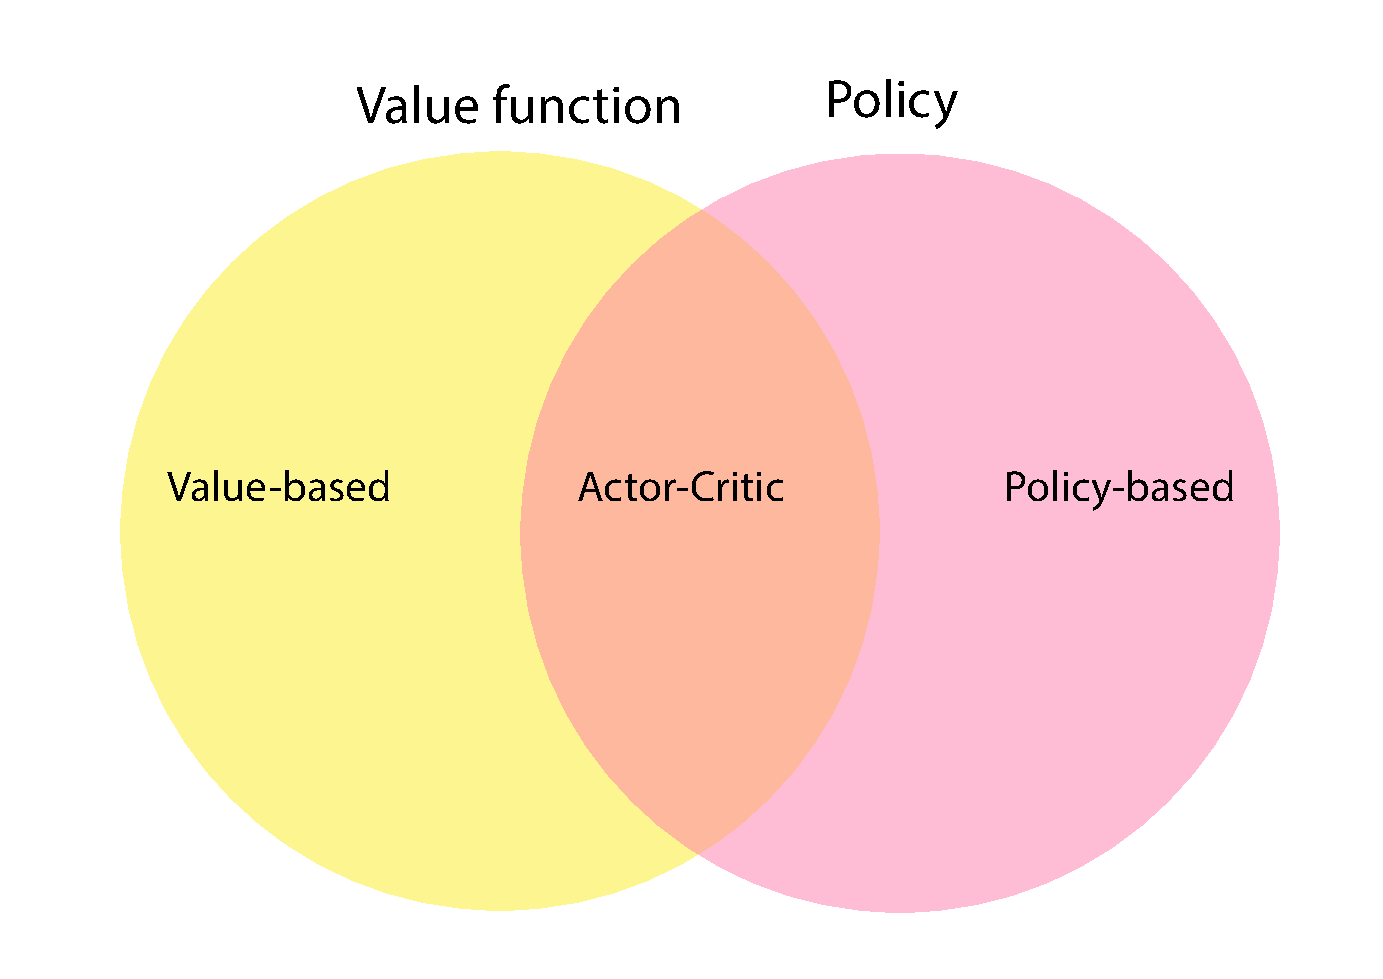
\includegraphics[width=80mm]{figures/valuepolicy.pdf}
\caption{Example of caption}
\label{fig:example}
\end{figure}


\subsection{Policy based methods}
We parameterize the policy with some unknown parameters $\theta$:

	\begin{equation}
	 	\pi (a|s, \theta) = \Pr \{A_t = s | S_t = s, \theta_t = \theta \}
	 \end{equation} 

Notice that in this course we will use $\theta$ for unknown parameters in policy and \textbf{w} for unknown parameters in value functions. The aim is to learn these parameters $\theta$ from experience. For this we need stochastic policies to get exploration. We will here assume that $\pi (a|s,\theta)$ is differentiable with respect to $\theta$. 

\begin{example}{Example: Soft-max policies (discrete action spaces)}
Soft-max policies can be used in discrete action spaces, if we let $h(s,a,\theta)$ denote our action preferences. We can create a distribution so that preferable actions have a high chance of getting picked:

	\begin{equation*}
		\pi (a|s,\theta) \propto e^{h(s,a,\theta)}
	\end{equation*}

Being more specific the probabilities: the probabilities will sum to 1. 

	\begin{equation}
		\pi (a|s,\theta) = \frac{e^{h(s,a,\theta)}} {\sum_{b}^{}e^{h(s,a,\theta)}} 
	\end{equation}

We can parametrize $h(s,a,\theta)$ either linear or non-linear. Where in the linear case we have: $h(s,a,\theta) = \theta^{T}x(s,a)$ and the non-linear being a neural network. 

\end{example}	

\subsection{Random continuous variables}
If we consider a scalar random continuous variable $a$. The probability density function $p(a)$ describes "the relative likelihood" that a random variable takes on different values:

	\begin{equation}
		\Pr \{ z_L \le a \le z_H\} = \int_{z_L}^{z_H} p(a)\,\text{d}a
	\end{equation}

The probability that $a$ takes on any value is 1 so: $\int_{-\infty}^{\infty} p(a)\,\text{d}a = 1$ and the expected value and variance are:

	\begin{equation}
	\begin{aligned}
		\mathbb{E} [a] = \mu = \int_{-\infty}^{\infty} ap(a)\,\text{d}a \\
		\text{var} [a] = \sigma^{2} = \mathbb{E}[(a-\mathbb{E}[a])^{2}]
	\end{aligned}
	\end{equation}


\begin{example}{Example: Gaussian polices (continuous action spaces)}
Gaussian policies can be used in continuous action spaces. If $a$ is a scalar variable we can use 

	\begin{equation}
		\pi (a|s,\theta) = \mathcal{N}(a; \mu(s,\theta),\sigma(s,\theta))
	\end{equation}
If a is multivariate, then we use the multi-variate Gaussian distribution instead.

	\begin{equation}
	\begin{aligned}
		\theta = \begin{bmatrix} \theta_\mu \\ \theta_\sigma \end{bmatrix} \\ \mu(s,a) = \theta_\mu^{T} X_\mu(s) \\ \sigma(s,\theta) = \exp(\theta_\sigma^{T}x_\sigma(s))
	\end{aligned}
	\end{equation}

In the case of a Neural network, it would take a as an input and output $\mu$ and $\sigma$

\end{example}	


\subsection{Why policy-based methods}
So why do we use policy-based methods? In order to deal with high-dimensional and continuous action spaces directly. We can by using these methods incorporate prior knowledge of the problem. It is possible to adjust the variance and thus also the exploration over time with these methods. Previously we have used for example $\epsilon$-greedy for exploration, but in policy-based the agent can start of by exploring very randomly but then over time adjust the parameters $\theta$ in order to approach a more deterministic optimal policy. Policy-based methods can also learn a stochastic policy. 

\subsection{Why have a stochastic policy?}
Then the question of: why having a stochastic policy arise. For a Markov decision process there will always be a deterministic optimal policy. For exploration it is possible to use $\epsilon$-greedy like discussed earlier, but this will not change the fact that the optimal policy is deterministic. However if we don't observe the full state s, then the optimal policy will not always be deterministic. One important case, if we use function approximation, in other words: $\hat{q}(s,a,\textbf{w}) = \textbf{w}^{T}\textbf{x}(s,a)$ then we only "see" the state through our features \textbf{x}$(s,a$ and may actually lose information ("State-aliasing")


\subsection{Policy-gradient methods}
If we let $J(\theta): \mathbb{R}^{d} \rightarrow \mathbb{R}$ be a scalar valued function with a vector input. We aim to find $\theta$ that \emph{maximizes} $J(\theta)$. For this we can use the gradient:

	\begin{equation}
	 	\nabla J(\theta) := \frac{\partial J} {\partial \theta} := \begin{bmatrix} \frac{\partial J} {\partial \theta_1} \\ \vdots \\ \frac{\partial J} {\partial \theta_d}   \end{bmatrix} \in \mathbb{R}^{d}
	 \end{equation}

At a point $\overline{\theta}, J(\theta)$ increases fastest in the direction $+\nabla J(\hat{\theta})$  and the gradient ascent will there for be: $\theta \leftarrow \theta + \alpha J(\theta), \quad \alpha > 0$

\subsection{What criterion to maximize?}
We will here for simplicity assume that $\gamma = 1$, in other words no discount, so that the return will be $G_t = \sum_{k= t+1}^{T} R_k$. In the RL course literature it is focused on episodic environments starting in $s_0$ and use:

	\begin{equation}
		J(\theta) = v_{\pi_\theta} (s_0) = \mathbb{E}[G_0 |S_0 = s_0]
	\end{equation}

Other criteria will give a similar result, in other words, the \emph{average value}
	\begin{equation}
		J(\theta) = \sum_{s}^{}\mu_{\pi_\theta}(s)v_{\pi_\theta}(s)
	\end{equation}
Here we encounter a challenge, a change in $\theta$ will affect:

\begin{itemize}
	\item Action selection: Since $\pi (a|s,\theta)$ is known, we know how the changes in $\theta$ affects the action selection
	\item State distribution: However, how a change in $\theta$ affects the state distribution depends on the \emph{unknown environment}
\end{itemize}

\begin{example}{Example: One-step MDP}
	\begin{itemize}
		\item Random starting state $s \sim d(s)$
		\item Terminating after one action with the reward distribution $p(r|s,a)$ 
		\item \textbf{State-values:} since the next state is always terminating
			\begin{equation}
				v_{\pi_\theta} = \mathbb{E}[R_1 |S_0 =s] = \sum_{a}^{}\pi (a|s,\theta)q(s,a)
			\end{equation}
		\item \textbf{Action-values:}
			\begin{equation}
				q(s,a) = \mathbb{E}[R_1 |S_0 = s, A_0 = a] = \sum_{r}^{}r p(r|s,a) \pi (a|s,\theta)d(s)
			\end{equation}
			Note that the action-values do not depend on the policy, since the next state is always terminating! This is NOT true for general MDP
		\item \textbf{Criterion} to maximize
			\begin{equation}
			\begin{aligned}
				J(\theta) = \mathbb{E}_{\pi_\theta}[v_{\pi_\theta}(s)] = \sum_{s}^{}d(s)v_{\pi_\theta}(s) = \sum_{s,a,r}^{} r p(r|s,a)\pi (a|s,\theta)d(s) \\ J (\theta) = \mathbb{E}_{\pi_\theta} [v_{\pi_\theta}(s)] = \sum_{s,a,r}^{} p(r|s,a)\pi (a|s,\theta)d(s) \\
				\nabla J(\theta) = \sum_{s,a,r}^{}[r \nabla \pi (a|s, \theta)] p(r|s,a)d(s)\\
				= \sum_{s,a,r}^{} [ r\frac{\nabla \pi (a|s,\theta)} {\pi (a|s,\theta)} ] p(r|s,a) \pi (a|s,\theta)d(s) \\
				= \sum_{s,a,r}^{} [r \nabla \ln \pi (a|s,\theta)]p(r|s,a) \pi (a|s,\theta)d(s) \\
				= \mathbb{E}_{\pi_\theta} [R_1 \nabla \ln \pi (A_0|S_0, \theta)]
			\end{aligned}
			\end{equation}
		In the third equality we used : $\nabla \ln f(\theta) = \frac{\nabla f(\theta)} {f(\theta)} $
		\item \textbf{Stochastic gradient ascent:} Run with the policy $\pi_\theta$ to get $S_0, A_0, R_1$ and update:
			\begin{equation}
				\theta \leftarrow \theta + \alpha G_t \nabla \ln \pi (A_0|S_0, \theta)
			\end{equation}
	\end{itemize}
\end{example}	


\subsection{The policy gradient theorem}
We now consider a general Markov decision process MDP again and let the criterion we want our policy to maximize to be: $J(\theta) = v_{\pi_\theta} (s_0)$

\begin{wbox}{The policy gradient theorem}
If $\pi (a|s, \theta)$ is differentiable, then:

	\begin{equation}
		\nabla J(\theta) = \mathbb{E}_{\pi_\theta} [q_{\pi_\theta}(S_t,A_t)\nabla \ln \pi (A_t|S_t, \theta)] = \mathbb{E}_{\pi_\theta} [G_t \nabla \ln \pi (A_t|S_t, \theta)],
	\end{equation}

here the second equality follows since $\mathbb{E}_{\pi_\theta} [G_t |S_t,A_t] = q_{\pi_\theta}(S_t,A_t)$
\end{wbox}


\subsection{Stochastic policy-gradient ascent (REINFORCE)}
	\begin{equation}
		\nabla J(\theta) = \mathbb{E}_{\pi_\theta} [q_{\pi_\theta}(S_t,A_t)\nabla \ln \pi (A_t|S_t, \theta)] = \mathbb{E}_{\pi_\theta} [G_t \nabla \ln \pi (A_t|S_t, \theta)],
	\end{equation}

The Reinforce update will be:

	\begin{equation}
	\begin{aligned}
		\theta \leftarrow \theta + \alpha G_t \nabla \ln \pi (A_t|S_t, \theta) \\
		= \theta + \alpha G_t \frac{\nabla \pi (A_t|S_t, \theta)} {\pi (A_t|S_t, \theta) } 
	\end{aligned}
	\end{equation}

The \textbf{interpretation:} $\nabla \pi (A_t|S_t, \theta)$ is the direction which we should change $\theta$ in to get most increase in the probability of taking action $A_t$ in state $S_t$. Each update scale this direction so that:

	\begin{itemize}
		\item Proportional to $G_t$
		\item Inversely proportional to the current probability of the action.
	\end{itemize}


The REINFORCE update has good theoretical convergence properties. The expected value of update equals the true gradient descent. It has high variance which may lead to slow learning, it is a Monte-Carlo method.

\begin{wbox}{REINFORCE}


\begin{itemize}
	\item Choose differentiable policy parametrization $\pi (a|s,\theta)$
	\item Initialize $\theta$
	\item \textbf{Loop:}
	\begin{itemize}
	 	\item Follow $\pi (a|s,\theta)$ to generate an episode trajectory $S_0,A_0,R_1,S_1,A_1,\ldots,S_{T-1},A_{T-1},R_T$
	 	\item For each time step t in the episode:
	 	\begin{itemize}
	 		\item $G_t = \sum_{k=t+1}^{T}R_k$
	 		\item $\theta \leftarrow \theta + \alpha G_t \nabla \ln \pi (A_t|S_t,\theta)$
	 	\end{itemize}
	 \end{itemize} 
This pseudo code is for $\gamma = 1$
\end{itemize}


\end{wbox}

 
    % end lectures
\end{document}  